\documentclass[tikz,border=8pt]{standalone}
\usepackage[utf8]{inputenc}
\usepackage{amsmath,amssymb}
\usepackage{microtype}
\usetikzlibrary{arrows.meta,calc,decorations.pathmorphing,positioning}

\definecolor{maroon}{RGB}{122,36,53}
\definecolor{taupe}{RGB}{124,95,88}
\definecolor{gold}{RGB}{154,106,31}
\definecolor{muted}{RGB}{124,116,104}
\definecolor{rule}{RGB}{189,169,132}

\begin{document}
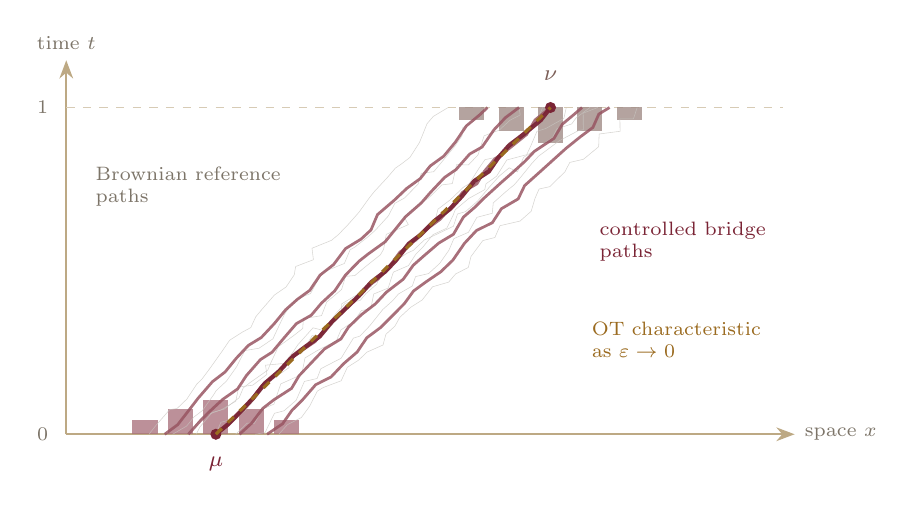
\begin{tikzpicture}[font=\small,>=Stealth,x=1cm,y=1cm]
  \draw[->,line width=0.8pt,rule] (0,0) -- (9.25,0)
    node[right,font=\scriptsize,muted] {space $x$};
  \draw[->,line width=0.8pt,rule] (0,0) -- (0,4.75)
    node[above,font=\scriptsize,muted] {time $t$};
  \draw[rule!60,dashed,thin] (0,4.15) -- (9.1,4.15);
  \node[muted,font=\scriptsize,left=3pt] at (0,0) {$0$};
  \node[muted,font=\scriptsize,left=3pt] at (0,4.15) {$1$};

  \foreach \x/\h in {1.0/0.55,1.45/1.0,1.9/1.35,2.35/1.0,2.8/0.55}{
    \fill[maroon!65,opacity=0.78]
      (\x-0.16,0) rectangle (\x+0.16,{0.32*\h});
  }
  \node[maroon,font=\footnotesize\bfseries] at (1.9,-0.38) {$\mu$};

  \foreach \x/\h in {5.15/0.5,5.65/0.95,6.15/1.4,6.65/0.95,7.15/0.5}{
    \fill[taupe!72,opacity=0.8]
      (\x-0.16,4.15) rectangle (\x+0.16,{4.15-0.32*\h});
  }
  \node[taupe,font=\footnotesize\bfseries] at (6.15,4.55) {$\nu$};

  \foreach \seed/\xs/\xt in {
    1/1.05/4.85,2/1.35/5.35,3/1.65/5.75,4/1.90/6.05,
    5/2.15/6.35,6/2.40/6.75,7/2.70/7.25,8/1.55/6.65}{
    \pgfmathsetseed{\seed}
    \draw[muted!42,very thin,opacity=0.72,
      decorate,decoration={random steps,segment length=4.8pt,amplitude=2.2pt}]
      (\xs,0) -- (\xt,4.15);
  }

  \foreach \seed/\xs/\xt in {
    21/1.25/5.35,22/1.55/5.75,23/1.90/6.15,
    24/2.20/6.55,25/2.55/6.90}{
    \pgfmathsetseed{\seed}
    \draw[maroon!78,line width=1.0pt,opacity=0.84,
      decorate,decoration={random steps,segment length=6.2pt,amplitude=1.15pt}]
      (\xs,0) -- (\xt,4.15);
  }

  \pgfmathsetseed{23}
  \draw[maroon,line width=1.55pt,opacity=0.96,
    decorate,decoration={random steps,segment length=6.5pt,amplitude=0.95pt}]
    (1.90,0) -- (6.15,4.15);
  \fill[maroon] (1.90,0) circle (2pt);
  \fill[maroon] (6.15,4.15) circle (2pt);
  \draw[gold,dashed,line width=1.15pt] (1.90,0) -- (6.15,4.15);

  \node[muted,font=\scriptsize,align=left,text width=2.35cm,anchor=west]
    at (0.25,3.15) {Brownian reference paths};
  \node[maroon,font=\scriptsize,align=left,text width=2.25cm,anchor=west]
    at (6.65,2.45) {controlled bridge paths};
  \node[gold,font=\scriptsize,align=left,text width=2.3cm,anchor=west]
    at (6.55,1.2) {OT characteristic\\as $\varepsilon\to0$};
\end{tikzpicture}
\end{document}
